\documentclass[tikz,border=0pt,crop=true]{standalone}

\usepackage{tikz} % Allows creation of tikz pictures
\usepackage{varwidth}
\usetikzlibrary{arrows,shapes}

\begin{document}
    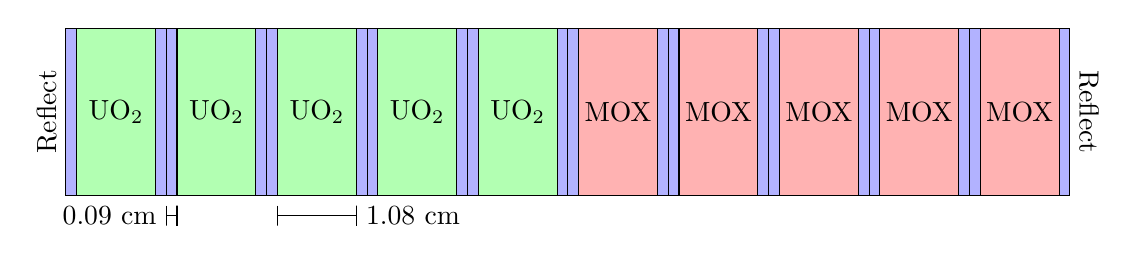
\begin{tikzpicture}[scale=0.85, every node/.style={scale=1}]
        \foreach \x in {0,1.5,...,6}
        \filldraw[xshift=\x cm, fill=green!30!white, draw=black] (0.160714286,0) 
        rectangle (1.339285714,2.5) node[pos=.5] {UO$_2$};
        \foreach \x in {7.5,9,...,13.5}
        \filldraw[xshift=\x cm, fill=red!30!white, draw=black] (0.160714286,0) 
        rectangle (1.339285714,2.5) node[pos=.5] {MOX};
        \foreach \x in {0,1.5,...,13.5}
        \filldraw[xshift=\x cm, fill=blue!30!white, draw=black] (0,0) rectangle 
        (0.160714286,2.5);
        \foreach \x in {0,1.5,...,13.5}
        \filldraw[xshift=\x cm, fill=blue!30!white, draw=black] (1.339285714,0) 
        rectangle (1.5,2.5);
        \draw[xshift=15cm,yshift=1.25cm] node[right] {\rotatebox{-90}{Reflect}};
        \draw[yshift=1.25cm] node[left] {\rotatebox{90}{Reflect}};
        \draw (1.5,-.15) -- (1.5,-.45) -- (1.5,-.30) node[left] {0.09 cm} -- 
        (1.660714286,-.30) -- (1.660714286,-.15) -- (1.660714286, -.45);
        \draw (3.160714286,-.15) -- (3.160714286,-.45) -- (3.160714286,-.30) -- 
        (4.339285714,-.30) node[right] {1.08 cm} -- (4.339285714,-.15) -- 
        (4.339285714, -.45);
    \end{tikzpicture}
\end{document}
